\documentclass{report}
% \documentclass{article}
% Language
\usepackage[T1]{fontenc}
\usepackage[utf8]{inputenc}
\usepackage[english]{babel}

% Page formatting
\usepackage{geometry}
\geometry{a4paper, margin=25mm, includefoot}

% Font, line height, paragraph indentation
% \usepackage{mathptmx} % Times New Roman
\usepackage{newtxtext, newtxmath} % Times New Roman (Modern + Math symbols)
\linespread{1.2}
\setlength{\parindent}{0pt}
% \usepackage{setspace}

% Chapter/section title formatting
\usepackage{titlesec}
\titleformat{\chapter}[display]{\normalfont\Large}{\chaptertitlename\ \thechapter}{0pt}{\huge\bfseries}[\vspace{8pt}\titlerule]
\titlespacing{\chapter}{0cm}{0cm}{0.5cm}

\titleformat{\paragraph}
{\normalfont\normalsize\bfseries}{\theparagraph}{1em}{}
\titlespacing*{\paragraph}
{0pt}{3.25ex plus 1ex minus .2ex}{1.5ex plus .2ex}

% Multi-column TOC
\usepackage{multicol}
% \makeatletter
% \renewcommand{\tableofcontents}[1][\contentsname]{%
%     \chapter*{#1}
%     \begin{small}
%     % \setlength{\columnseprule}{0.5pt}
%     \setlength{\columnsep}{20pt}
%     \begin{multicols}{2}
%         \@starttoc{toc}
%     \end{multicols}
%     \end{small}
% }
% \makeatother

% Used for moving abstract from the center of the page to the top
\usepackage{etoolbox}
\patchcmd{\abstract}{\null\vfil}{}{}{}

% Figures and captions
% \usepackage{caption}
\usepackage{float}
\usepackage{graphicx}
\usepackage{wrapfig}
\usepackage[font=small,labelfont=bf]{caption}
\usepackage[labelformat=simple]{subcaption}
\renewcommand\thesubfigure{(\alph{subfigure})}

\def \FigureAbbreviaition {Fig.}
\newcommand{\figref}[1]{\FigureAbbreviaition\ \ref{#1}}
\newcommand{\tabref}[1]{Table \ref{#1}}
\newcommand{\chapref}[1]{Chapter \ref{#1}}

% Figure caption formatting
\AtBeginDocument{%
\captionsetup[figure]{name={\FigureAbbreviaition},aboveskip=10pt,belowskip=-10pt}
\captionsetup[subfigure]{aboveskip=10pt,belowskip=0pt}
\captionsetup[table]{aboveskip=10pt,belowskip=-10pt}
% \captionsetup[subtable]{aboveskip=10pt,belowskip=0pt}
}

% Array
\usepackage{array}
\usepackage{textpos}

% Math and symbols
% \usepackage{amsmath, amssymb, bm} % newtxmath has same defines as amssymb

\usepackage{amsmath}
\newtheorem{problem}{Problem}

% \theoremstyle{remark}

\usepackage{amsmath, bm}
\usepackage{mathtools}
\usepackage{verbatim}
\usepackage{xfrac}
\usepackage{tensor}
\usepackage{interval}
\usepackage{commath} % for \abs, \norm
\usepackage{physics} % for qty(), qty{} etc. (automatic parentheses)

% Custom commands
\usepackage{xstring}
\usepackage{xspace}




\newcommand{\fakecite}[0]{\hl{\textbackslash cite}\xspace}
\renewcommand{\vec}[1]{\ensuremath{\bm{#1}}} % vector [amsmath, bm]
\newcommand{\mat}[1]{\ensuremath{\bm{\mathrm{#1}}}} % matrix [amsmath, bm]
\newcommand{\T}[0]{\ensuremath{^\mathsf{T}}} % transpose ^T
\newcommand{\inv}[0]{\ensuremath{^{-1}}} % inverse ^{-1}
\newcommand{\pinv}[0]{\ensuremath{^{\dagger}}} % pseudo-inverse ^{-1}
\newcommand{\rvec}[1]{\ensuremath{\renewcommand{\arraystretch}{0.6}\begin{bmatrix} #1 \end{bmatrix}}}
\newcommand{\cvec}[1]{\ensuremath{\renewcommand{\arraystretch}{1.0}\begin{bmatrix} #1 \end{bmatrix}}}
\newcommand{\twodots}{\mathinner {\ldotp \ldotp}} % .. (two dots)
\renewcommand{\secref}[1]{\hyperref[#1]{\ref*{#1}\ \nameref*{#1}}}
% \newcommand{\tf}[3][T]{\ensuremath{\tensor[^{#2}]{\mat{#1}}{_{#3}}}}
\newcommand{\tf}[3][T]{\ensuremath{{\mat{#1}^{#2}_{#3}}}}
\newcommand{\highlight}[1]{\hl{#1}\xspace}
\newcommand*\of{\qty} % $f\of(x)$

% usage: \tf{from}{to} | \tf[T]{from}{to} | \tf[R]{from}{to} | \tf[t]{from}{to} etc.
% \newcommand{\tf}[3][T]{%
%     \IfEqCase{#1}{%
%         {T}{\ensuremath{\tensor[^{#2}]{\mat{#1}}{_{#3}}}}%
%         {R}{\ensuremath{\tensor[^{#2}]{\mat{#1}}{_{#3}}}}%
%         {t}{\ensuremath{\tensor[^{#2}]{\vec{#1}}{_{#3}}}}%
%         {p}{\ensuremath{\tensor[^{#2}]{\vec{#1}}{_{#3}}}}%
%     }[\PackageError{tf}{Undefined option: #1}{}]%
% }%

% Equation spacing
\AtBeginDocument{%
\abovedisplayskip=6pt plus 2pt minus 2pt
\abovedisplayshortskip=6pt plus 2pt minus 2pt
\belowdisplayskip=6pt plus 2pt minus 2pt
\belowdisplayshortskip=6pt plus 2pt minus 2pt
}

% SI units + config and custom units
\usepackage{siunitx}[=v2]
\sisetup{
    per-mode=fraction, fraction-function=\sfrac, % fractions
    % round-mode=figures, round-precision=3, % rounding
    output-exponent-marker=\ensuremath{\mathrm{e}},
    separate-uncertainty=true, multi-part-units=single, % for \SI{2 \pm 0.2}{\rad},
    binary-units=true, % for \byte, \giga etc.
}
\DeclareSIUnit \pixel {px}

% Text highlight (\hl)
\usepackage{soul}

% Enumeration and tables
\usepackage{enumerate}
\usepackage{enumitem}
\usepackage{multirow} 
\usepackage{multicol}
\usepackage{ltablex}
\usepackage{spreadtab}
\usepackage{booktabs}
\usepackage{tabto}

\usepackage{diagbox}
\usepackage{tabularx}
\usepackage[export]{adjustbox}

% Custom tables commands for fixed-column sizes
\newcommand{\PreserveBackslash}[1]{\let\temp=\\#1\let\\=\temp}
\newcolumntype{C}[1]{>{\PreserveBackslash\centering}p{#1}}
\newcolumntype{R}[1]{>{\PreserveBackslash\raggedleft}p{#1}}
\newcolumntype{L}[1]{>{\PreserveBackslash\raggedright}p{#1}}

\setlength\doublerulesep{0.3cm} % when using a double line, make extra space

% Enumeration formatting
\newcommand{\tabitem}{~~\llap{\textbullet}~~}
\newcommand{\sqrbulletsml}{\textcolor{black}{\raisebox{.45ex}{\rule{.6ex}{.6ex}}}}
\newcommand{\sqrbulletmed}{\textcolor{black}{\raisebox{.40ex}{\rule{.7ex}{.7ex}}}}

\renewcommand{\labelitemi}{\sqrbulletmed}
\renewcommand{\labelitemii}{\sqrbulletsml}
\renewcommand{\labelitemiii}{\sqrbulletsml}
\renewcommand{\labelitemiv}{\sqrbulletsml}

% Colors (latexcolor.com)
\usepackage[table]{xcolor}
\definecolor{cerulean}{rgb}{0.0, 0.48, 0.65}
\definecolor{earthyellow}{rgb}{0.88, 0.66, 0.37}
\definecolor{darkmagenta}{rgb}{0.55, 0.0, 0.55}
\definecolor{darkolivegreen}{rgb}{0.33, 0.42, 0.18}
\definecolor{codegray}{gray}{0.9}
\definecolor{gainsboro}{rgb}{0.86, 0.86, 0.86}
\definecolor{cyan}{rgb}{0.0, 1.0, 1.0}

\definecolor{light-yellow}{RGB}{255, 255, 137}
\definecolor{light-blue}{RGB}{148, 201, 233}

\definecolor{tableheader}{gray}{0.9}

\definecolor{metaorange}{rgb}{0.98, 0.54, 0.13} % also known as flame orange

% colored square box
% https://tex.stackexchange.com/questions/201300/inline-boxes-alternative-to-pifonts-non-filled-but-shadowed-box
\newcommand{\sqbox}[1]{\textcolor{#1}{\rule{1.2ex}{1.2ex}}}

% Code snippets
\usepackage{listings}
% \renewcommand{\arraystretch}{1.2}
\renewcommand{\tabcolsep}{0.2cm}

% Code snippets formatting
\lstset{
    backgroundcolor=\color{black!5},        % set backgroundcolor
    basicstyle=\footnotesize\ttfamily,      % basic font setting
    captionpos=b,                           % caption position
    frame=single,                           % draw a frame at the top and bottom of the code block
    framesep=5pt,                           % frame margin
    xleftmargin=5pt,                        % frame margin
    xrightmargin=5pt,                       % frame margin
    tabsize=4,                              % tab space width
    showstringspaces=false,                 % don't mark spaces in strings
    breaklines=true,                        % wrap lines
    commentstyle=\color{darkolivegreen},    % comment color
    keywordstyle=\color{darkmagenta},       % keyword color
    stringstyle=\color{earthyellow},        % string color
    identifierstyle=\color{cerulean},
}

% Custom inline-code command (\code)
%\newcommand{\lstinln}[1]{\colorbox{gainsboro}{\texttt{#1}}}
\newcommand{\code}[1]{%
  \begingroup\setlength{\fboxsep}{2pt}%
  \colorbox{gainsboro}{\texttt{\hspace{2pt}\vphantom{Ay}#1\hspace{2pt}}}%
  \endgroup
}

% package labels
\usepackage{tikz}
\newcommand{\meta}[1]{ \tikz[baseline=(X.base)]\node [draw=metaorange,fill=metaorange,semithick,rectangle,inner sep=2.5pt, rounded corners=2pt] (X) {  \textbf{\textcolor{white}{\textsf{#1}}}}; \hphantom}
\newcommand{\pkg}[1] { \tikz[baseline=(X.base)]\node [draw=blue,fill=blue,semithick,rectangle,inner sep=1.3pt, rounded corners=2pt] (X)             {  \textbf{\textcolor{white}{\textsf{#1}}}}; \hphantom}




% Appendices
\usepackage[toc]{appendix}

% Bibliography and citation
\usepackage[style=numeric, sorting=none]{biblatex}
\usepackage{csquotes}
\DeclareNameAlias{sortname}{family-given}
\DeclareNameAlias{default}{family-given}

\addbibresource{resources.bib}

% Section cross-referencing
\usepackage{nameref}
\usepackage{hyperref}

% Label counter formatting (e.g. Figure 1 or Figure 2.1)
% In case you want the numbering to to start with the chapter number e.g. 1.1 1.2 1.3 for chapter 1 figures, use this instead of the one below
\usepackage{chngcntr} 
\AtBeginDocument{%
    \counterwithin{figure}{chapter}
    \counterwithin{table}{chapter}
    \counterwithin{equation}{chapter}
    \counterwithin{lstlisting}{chapter}
}

% In case you want the numbering to continue between chapters e.g. 1 2 3 4 5, use this instead of the one above
% \usepackage{chngcntr} 
% \AtBeginDocument{%
%     \counterwithout{figure}{chapter}
%     \counterwithout{table}{chapter}
%     \counterwithout{equation}{chapter}
%     \counterwithout{lstlisting}{chapter}
% }

% Glossaries and acronyms
% must be loaded last + no empty includes in main document.
\usepackage[automake, acronym, nogroupskip, nonumberlist]{glossaries}
\usepackage{glossary-mcols}
\setglossarysection{section}

% command for dual entries
% \newdualentry[<options>]{<label>}{<abbrv>}{<long>}{<description>}
% https://tex.stackexchange.com/a/368666
\newcommand*{\newdualentry}[5][]{%
  \newglossaryentry{main-#2}{%
    name={#4 (\glslink{#2}{#3})},%
    text={#3\glsadd{#2}},%
    description={{#5}},%
    #1%
  }%
  \newglossaryentry{#2}{%
    type=\acronymtype,%
    first={\glslink{main-#2}{#4 (#3)}},%
    name={#3\glsadd{main-#2}},%
    description={\glslink{main-#2}{#4}},%
    plural={#2s},%
    firstplural={\glsentrydesc{#2}s (\glsentryplural{#2})}
  }%
}

% setup and load glossaries
\makeglossaries
\loadglsentries{glossary}

% only hyperlink first-time glossary entries
% \renewcommand*{\glslinkcheckfirsthyperhook}{%
%   \ifglsused{\glslabel}%
%   {%
%     \setkeys{glslink}{hyper=false}%
%   }%
%   {}%
% }

% generate word count text file wc.tex
\immediate\write18{bash wc.sh}

\begin{document}

% title page

\begin{titlepage}
    \begin{center}
   
        \vspace*{0.5cm}
        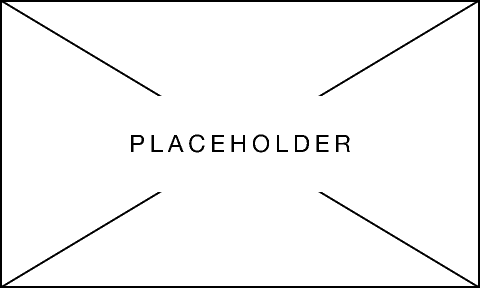
\includegraphics[width=5cm]{img/placeholder.png}
        \vspace{2cm}
        
        {\LARGE Some Placeholder Title \par}


        \vspace{1cm}
        \textbf{A Master Thesis}
        \vspace{0.5cm}
       
        written by
       
        \vspace{0.5cm}
        
        \begin{tabular}[t]{c@{\extracolsep{4em}}}
        \textbf{Name}\\
        my@email.dk\\
        potential-number \\
        \end{tabular}
        
        \vspace{8.0cm}
        
        \begin{center}
        The code for this project is available at\\
        \url{url-to-some-github}
        \end{center}
        
        \vfill
        
        \textbf{Overarching Institution}\\  
        Specific Department\\
        
        \vspace{0.5cm}
        
        Word Count : [some word count] \\
        Date of Hand In
        % \today
            
   \end{center}
\end{titlepage}

% preface
% \input{sections/0-preface}

% roman numbering for abstract, TOC, glossary etc.
\pagenumbering{roman}

% abstract
\clearpage
\begin{abstract}
\setlength{\parindent}{0pt}
\normalsize

% \noindent Some abstract text explaining the goal, methods and conclusion of the project. \\

% This project presents a new \gls{pnp} pipeline by excluding the vision systems and using purely tactile inputs to eliminate the weaknesses of vision algorithms such as transparency and reflectance. To develop this pipeline three subproblems were identified: tactile perception, pose estimation and in-hand manipulation. Tactile perception consisted of estimating the contact point, normals and skew forces. Using physics engine assistance, all three quantities were succesfully estimated. The pose estimation was successfully achieved on synthetic data with an orientation error less than \SI{5}{\degree} and translation error less than \SI{1}{\centi\meter} at \SI{10}{\percent} outliers. The in-hand manipulation problem was successfully solved using \gls{dapg}, which entailed an analysis of the training process and end performance. Finally, potential improvements to the pipeline is discussed for future iterations.

In this project, a novel pipeline for a \gls{pnp} task is presented, focusing on utilizing tactile inputs instead of vision systems to overcome the limitations of vision algorithms, such as transparency and reflectance issues. The development of this pipeline involved addressing three key subproblems: \gls{tp}, \gls{pe}, and in-hand manipulation. \gls{tp} involved accurately estimating the contact points, contact normals, and skew forces. The contact normals were successfully estimated using \gls{rls}, the contact points were found using the grasp matrix, while a \gls{dl} model was attempted to be used for skew force estimation without success. To compensate for the missing skew forces and cases of contact normals assistance of the Gazebo physics engine was applied successfully. The \gls{pe} task demonstrated promising results on synthetic data using \gls{gnc} for outlier rejection and \gls{rcqp} for transformation estimation. This resulted in an orientation error of \num{3} degrees and a translation error of  \SI{0.08}{\centi\meter} while in the presence of \SI{10}{\percent} outliers, which was within the criteria for success. For the in-hand manipulation problem, the use of \gls{dapg} proved successful in the MuJoCo dynamic simulator, and a comprehensive analysis of the training process and final performance was conducted. Lastly, potential enhancements for future iterations of the pipeline are discussed.



\end{abstract}

% table of contents
\clearpage
\tableofcontents

% workload distribution
\clearpage

\section*{Acknowledgements}

I would like to express my sincere gratitude to those who have supported and guided me throughout my thesis project. \medskip

First and foremost, I would like to extend my deepest appreciation to my thesis supervisor, Christoffer Sloth, Lector at SDU Robotics, for his exceptional guidance and support throughout the entire process. His expertise and knowledge in the field of robotics have been invaluable in shaping this project. \medskip

I would also like to thank Yitaek Kim for his invaluable support and sparring in solving key aspects of this project. His insights and advice have been critical to the successful completion of this thesis. \medskip

Furthermore, I would like to extend my thanks to Shadow Robotics for providing the underlying software for the project to build upon along with technical support, enabling this project. Their contribution has been essential in the successful completion of this project. \medskip

Finally, I would like to thank my family and friends for their unwavering support and encouragement throughout this journey. Their love and support have been a constant source of motivation and inspiration. \medskip

Once again, I express my deepest gratitude to all those who have played a significant role in this project.

\addcontentsline{toc}{section}{Acknowledgments}

% glossary & acronyms
\clearpage
\addcontentsline{toc}{section}{Acronyms and Terms}
\printglossary[type=acronym, title=Acronyms, style=mcolindex]
\printglossary[type=main, title=Terms]

% main document
\clearpage
\pagenumbering{arabic}
\glsresetall

\pagebreak
\chapter{Example section}\label{ch:example}

This document demonstrate the use of figures, references, SI units, glossary, math notation, lists, and otherwise relevant formatting specifications. Paragraphs are typically separated using \texttt{\textbackslash medskip}.\medskip

\begin{figure}[H]
    \centering
    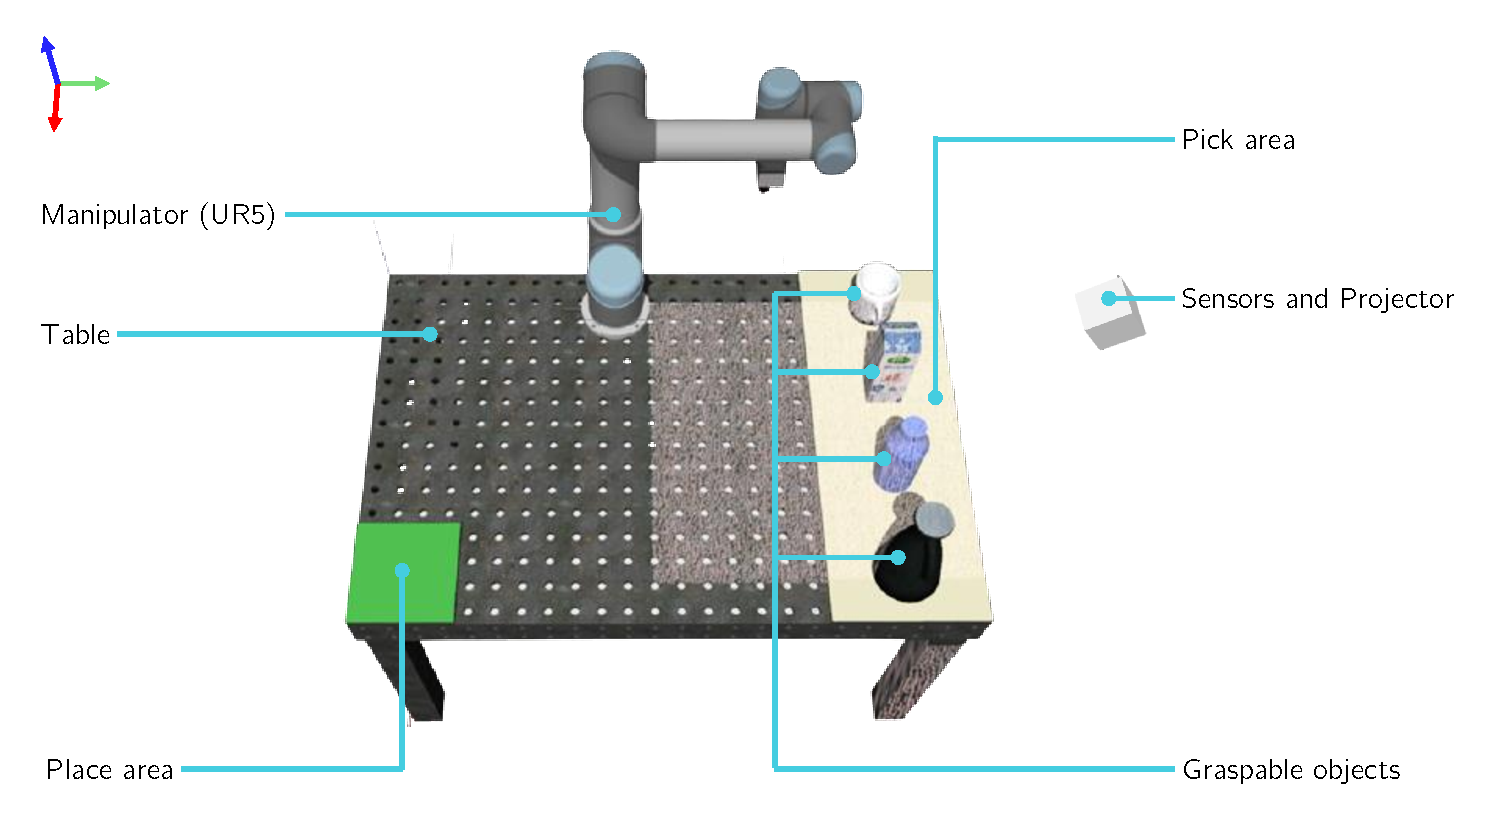
\includegraphics[width=.6\linewidth]{chapters/example/fig/figure.pdf}
    \caption{An example image using \acrlong{acronym-label}.}
    \label{fig:example-figure}
\end{figure}

To exemplify math notation, consider the mapping between the joint configuration of a robot
%
\begin{equation}
    \vec{q} = \rvec{q_1 & q_2 & \dots & q_n}\T,
    \label{eq:jnt-config}
\end{equation}

and \gls{glossary-label}, given as a homogeneous transformation
%
\begin{equation}
    \renewcommand{\arraystretch}{1.2}
    \tf{A}{B} = \begin{bmatrix}
        \tf[R]{A}{B}         & \tf[t]{A}{B} \\
        \vec{0}^{1 \times 3} & 1 
    \end{bmatrix},
\end{equation}

where \tf[R]{A}{B} and \tf[t]{A}{B} is the rotation and translation, respectively, from frame $\{A\}$ to frame $\{B\}$, denoted using a homogeneous transformation matrix $\mat{T}(\vec{q}) \in \mathbb{R}^{4 \times 4}$ as a function of the joint configuration in \eqref{eq:jnt-config}, as described in \cite{robotics-book}.\medskip

Complex table/figure hybrids with aligned captions and functioning labels can be implemented using \texttt{minipage}, as shown in \tabref{tab:example-table} and \figref{fig:example-plot}. Use \fakecite as a placeholder for citations.

\begin{center}
    \renewcommand{\arraystretch}{1.2}
    \begin{minipage}{.4\linewidth}
        \vspace{-10pt}
        \centering
        \begin{tabular}{|l|c|c|c|}
        \hline
        \diagbox[width=5.5em, font=\footnotesize\bfseries]{Method}{Pose} & 1 & 2 & 3 \\ \hline
        Linear    & \SI{18.97}{\second} & \SI{20.35}{\second} & \SI{22.85}{\second} \\ \hline
        Parabolic & \SI{13.66}{\second} & \SI{14.93}{\second} & \SI{17.33}{\second} \\ \hline
        \end{tabular}%
    \end{minipage}%
    \hfill%
    \begin{minipage}{.55\linewidth}
        \vspace{0pt}
        \centering
        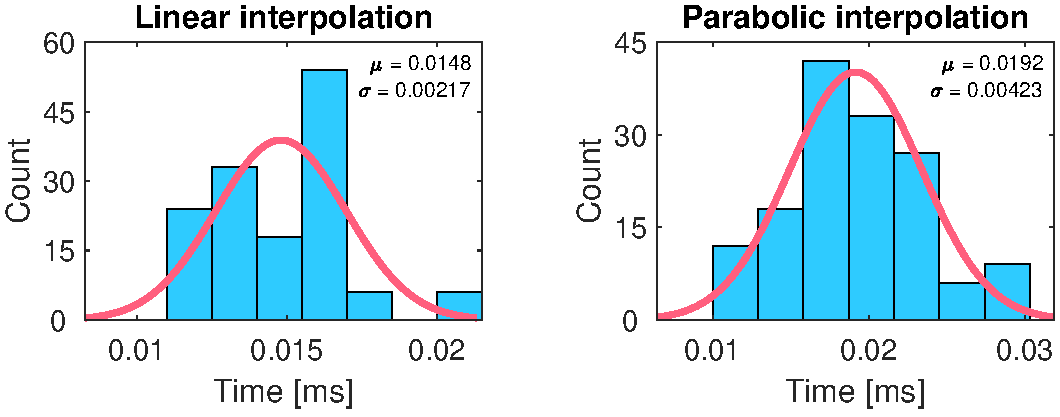
\includegraphics[width=.95\textwidth]{chapters/example/fig/plot.pdf}
    \end{minipage}%
    %    
    \vspace{15pt}
    %
    \begin{minipage}[t]{.4\linewidth}
        \vspace{0pt}
        \captionsetup{type=table}
        \captionof{table}{Trajectory durations of the interpolation-based trajectory generation methods.}
        \label{tab:example-table}
    \end{minipage}%
    \hfill%
    \begin{minipage}[t]{.55\linewidth}
        \vspace{0pt}
        \captionsetup{type=figure}
        \captionof{figure}{Average planning time for each of the interpolation-based trajectory generation methods.}
        \label{fig:example-plot}
    \end{minipage}%
\end{center}

For numbers, units and ranges, the \texttt{siunitx} package is used, which allows to express a number \num{10}, a range of \SIrange{5}{6}{\second}, or a SI unit of \SI{5.73 \pm 1.09}{\second}. Inline row-vectors (with the transpose symbol) can be written as $\vec{a} = \rvec{\vec{a}_p & \vec{a}_o}\T$, where as parentheses can be automatically written using $\qty(a, b)$ or $\qty{\frac{a}{b}, c}$. Also, shorthands for \mat{A}\inv, \mat{A}\pinv and \mat{A}\T.\medskip

\glsresetall

\pagebreak
\chapter{Introduction}\label{ch:intro}

\section{Context}\label{sec:intro-context}

% historical context
As of 2022 humanity has developed tools for unprecedented growth in wealth and technology on a global scale \fakecite. In such times a great deal of consumerism and interconnection is present with people needing product produced faster and more consistently than ever \fakecite. 
As one would expect, this creates a high demand for manufacturers to reliably and consistently being able to provide products, while also remaining flexible, as the demand for different product change rapidly. 
% argue for why automation is better
% https://www.fishmancorp.com/robotics-manufacturing/
% https://www.universal-robots.com/blog/solving-complex-problems-with-innovative-concepts-and-robotic-solutions/
In order to provide great volumes of products, manual labor has is essential as assembly, transport and manipulation processes rely on these. Due to these types of manual labor being largely done by unskilled workers, automation alternatives are being adopted which provides benefits. 
% this is referred to as industry 4.0
% benefits for employer
These include for the employer: Avoid having to pay monthly salaries to unskilled labored individuals doing manual tasks, here the automation solution only requires electrical energy and potential supervision by a qualified individual. Potential risks are also involved when hiring humans as the workforce can be inconsistent due to human error\fakecite or left out due to illness etc. Considerations with regards workers rights such as working conditions and wage also needs not to be considered. These cause production limitations in the form of stand still hours, such as bathroom and lunch breaks along with after work hours and holidays. 
% benefits for the employee 
This replacement of manual labor also benefits the employee, as boring and physically wearing work is automated, enabling the employees to take on different and less wearing roles. While the issue of labor unemployment becomes apparent solutions which provide support to already hired workers have been developed, such as \gls{cobot}\fakecite. \medskip

% categories of problems in robotics for factories
When implementing automation of production lines using robotics, certain categories of problems are revealed. These include: Assembly, alteration and \gls{pnp}, the last being the one of interest in this project. 
\section{Problem Description}\label{sec:intro-problem-description}
% applications
Pick and place \gls{manipulator}s are used in a wide variety of different fields such as 
sorting of waste \cite*{robotic-pick-and-toss-facilitates-urban-waste-sorting}
handling of food \cite*{automation-of-mobile-pick-and-place-robotic-system-for-small-food-industry}\cite*{development-of-a-food-handling-soft-robot-hand-considering-a-high-speed-pick-and-place-task} and factory bin picking \cite*{real-time-industrial-bin-picking-with-a-hybrid-deep-learning-engineering-approach} \cite*{a-bin-picking-benchmark-for-systematic-evaluation-of-robotic-pick-and-place-systems} \cite{generic-development-of-bin-pick-and-place-system-based-on-robot-operating-system}. The solutions in these industries are examples of subcategories under the pick and place problem, namely sorting and bin picking. Since both of these are sub categories of the pick and place problem, they fundamentally follow the same sequential four phases from start to end. 
% All of these problems fundamentally contain the same structure as shared among all pick-and-place problems.
These steps being pre-grasping, grasping, transport, and placement \cite*{a-bin-picking-benchmark-for-systematic-evaluation-of-robotic-pick-and-place-systems} for traditional .
% pre-grasp
The pre-grasp phase involves localizing the object(s), potentially estimating their pose and executing the trajectory to move the end effectors grasp, collision free to said object(s). Here different potential grasp can be considered in order to determine the best pose for the end effector.
% grasping
In the grasping phase the end effector gasps the object in such a manner that the object's entire weight is supported by the \gls{ee}, and ends when the object no longer is in contact with the environment, which often is the container holding the object.
% transport
The transportation phase involves the motion of the manipulator to move from the pose achieved after the grasping phase, to a pose ready for placement of the object in the desired placing area or fixture. Here considerations may be needed with regards to how much force and torque the \gls{ee} can tolerate without losing the object.
% placement
Finally the goal of the placing phase is to place the object within the placing area or fixture in a desired end pose. Here the constraints on the end pose might differ significantly based on the application, as the pose of greens in a crate might need less precision than if the manipulator hands a bolt to the next robotics system in the pipeline. \medskip

While these phases make up a traditional \gls{pnp} systems, certain assumptions are made regarding the objects of interest in order for this pipeline to function. Specifically the localization and pose estimation of the pre-grasp phase are assumed possible due to \gls{cv} often being the sensory system for such tasks. Due to \gls{cv} techniques mimicking the human eye the field's maturity has generated a wide range solution proposals to these problems.


solutions to computer vision: classical,old fashion, deep learning based 

deep learning on transparent objects and reflective objects, shown less than ideal results

classical approaches% https://ieeexplore.ieee.org/abstract/document/7860048


vision has been used for many years \fakecite 


% traditional pipeline makes assumptions -> 

% ind end effector pose est
\section{Thesis Overview}\label{sec:intro-thesis-overview}































































% The developments in robotics as a field has over the past years provided automation solutions to execute repetitive manual tasks with high efficiency and reliability \fakecite. One of the most common tasks being pick and place tasks which involves picking un an object from one position and placing is in another. This is can be parted into the following subparts: Object localization, pose estimation, grasping and placing. In the solutions currently present for industrial use \gls{cv} is used for object localization and \gls{pe} due to the low cost of cameras and the fields maturity. However, while these solutions may be sufficient for certain tasks they fundamentally suffer from the weaknesses introduced by vision techniques. These include a great number of outliers caused by occlusions, reflecting, transparent or homogeneous surfaces, and repetitive structures when solving the \gls{corr-problem}. These problems as of the writing of this project have jet to be completely solved. Promising results have been found with the rise of \gls{dl} which in present time has proven its versatility and provides proof of concept solutions for narrow cases in pose estimation of transparent \cite{6dof-pose-estimation-of-transparent-object-from-a-single-rgb-d-image} and reflective \medskip

% \begin{minipage}{0.45\textwidth}
% 	objects \cite{6d-pose-estimation-of-objects:-recent-technologies-and-challenges}. This is relevant since industrial settings often contain transparent and especially reflecting objects as metallic parts tend to appear frequently and have high reflectances. To solve these problems this project aims to perform in-hand pose estimation through only the use of tactile sensors. Specifically this will be done on a Shadow Dexterous Hand \cite{shadow-dex-hand} with 20 \gls{dof}. Using tactile inputs rather than visual, eliminates the weaknesses mentioned above. A schematic showing the hand can be seen in \figref{fig:shadow-dex-hand-schematic}. Using this approach, the overall problem can be partitioned into 3 sub-problems labeled problem 1, 2 and 3. Problem 1 involves modeling the contact between the gripper's fingers and the object, also referred to as tactile perception. Problem 2 is to convert the collected data from problem 1 to meaningful surface data, treat these data as features and use them to estimate pose candidates. Finally problem 3 involves in-hand manipulation, such that further information is gained by probing the object. Here new desired surface points are found through intelligent probing such that strong surface features are found to better identify the object's correct pose. \medskip
% 	\end{minipage} 
% 	\hfill
% 	\begin{minipage}{0.45\textwidth}
% 	\begin{figure}[H]
% 		\begin{small}
% 			\begin{center}
% 				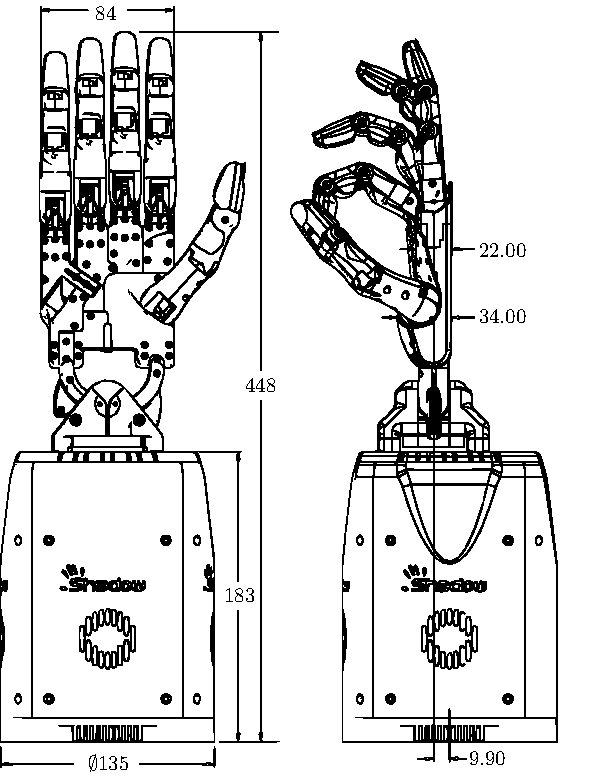
\includegraphics[width=0.95\textwidth]{chapters/introduction/fig/shadow-dex-hand-vector.pdf}
% 			\end{center}
% 			\caption{Schematic of Shadow Dexterous Hand from Shadow Robots, based on \cite{shadow-dex-hand-schematic}. The measurements are in \SI{}{\milli\metre}.}
% 			\label{fig:shadow-dex-hand-schematic}
% 		\end{small}
% 	\end{figure}
% \end{minipage}

% Thus the hypothesis of this projects $\text{H}_1$, will be testing if intelligent probing for strong features increases in-hand pose estimation performance, with the null hypothesis $\text{H}_0$ being that there is no statistical significant difference in the pose estimation performance of the system if the probing is done randomly or intelligently at a certainty level of \highlight{95\%}. Here pose estimation performance is quantified in terms of mean execution time for estimating the pose with an accuracy greater than \highlight{95\%}. \medskip

% The development of this project is done in the \gls{docker} provided by Shadow Robotics for simulation, control and development of the hand \cite{shadow-dex-github}. Here a hardware-simulation agnostic \gls{ros} \cite{ros} control \cite{ros-control} interface is found, which contains fundamental tools to interact with the robot hand. The dynamic simulation environment Gazebo \cite{gazebo} is likewise packaged as part of the \gls{docker} and is thus the one used for this project.
% To solve the problems presented, the \gls{ros} packages in \tabref{tab:software-package-table} will be applied, where \texttt{ros\_utils} and \texttt{in\_hand\_pose\_estimation} will be developed during this project.

% \begin{table}[h]
% 	\begin{small}
% 		\begin{center}
% 			\begin{tabular}[c]{ | l r | l | } \hline
% 				\cellcolor{tableheader} \textbf{Package}           & \cellcolor{tableheader} & \multicolumn{1}{l|}{\cellcolor{tableheader} \textbf{Description}} \\ \hline \hline
% 				\texttt{in\_hand\_pose\_estimation}                & \meta{meta} & \textbf{Project package of the in-hand pose estimation system} \\ \hline
% 				\hspace{0.3cm} \texttt{in\_hand\_pose\_estimation} &             & Integration of the full in-hand pose estimation pipeline  \\ \hline
% 				\hspace{0.3cm} \texttt{sr\_tactile\_image}         & \pkg{pkg}   & Extraction of tactile perception  \\ \hline
% 				\hspace{0.3cm} \texttt{sr\_pose\_estiamtion}       & \pkg{pkg}   & Estimate the pose of object based on tactile perception \\ \hline
% 				\hspace{0.3cm} \texttt{sr\_hand\_manipulation}     & \pkg{pkg}   & Manipulate object in hand to probe for strong features \\ \hline \hline
% 				\texttt{sr\_common}                                & \meta{meta} & \textbf{Shadow package for commonly used tools} \\ \hline
% 				\hspace{0.3cm} \texttt{sr\_common}                 &             & Implements commonly used tools such as messages \\ \hline
% 				\hspace{0.3cm} \texttt{sr\_robot\_msgs}            & \pkg{pkg}   & Messages used to communicate with the robot hand  \\ \hline 
% 				\hspace{0.3cm} \texttt{\dots}                      &             &  \\ \hline \hline
% 				\texttt{sr\_core}                                  & \meta{meta} & \textbf{Shadow package for core tools} \\ \hline
% 				\hspace{0.3cm} \texttt{sr\_core}                   &             & Implements core features of the hand such as hardware interfacing \\ \hline
% 				\hspace{0.3cm} \texttt{sr\_hand}                   & \pkg{pkg}   & Contains the hand commander for controlling the robot hand  \\ \hline
% 				\hspace{0.3cm} \texttt{\dots}                      &             &  \\ \hline \hline
% 				\texttt{ros\_utils}                                & \pkg{pkg}   & \textbf{Utilities for interfacing ROS/Gazebo/MoveIt/Eigen etc} \\ \hline
% 			\end{tabular}
% 		\end{center}
% 		\caption{Software packages used in the in-hand pose estimation system.}
% 		\label{tab:software-package-table}
% 	\end{small}
% \end{table}

% To present this work, the \gls{sota} solutions to each of the three problems described above will be presented in \chapref{ch:state-of-the-art}, where the best fitting methods for this use case will be chosen. In \chapref{ch:1-tactile-perception} to \chapref{ch:3-in-hand-manipulation} these solutions will be presented, analyzed, and their performance discussed and concluded upon. In \chapref{ch:4-system-integration} the system integration will be presented and the total performance of the system will be concluded. Finally in \chapref{ch:discussion} and \chapref{ch:conclusion} the results and methods will be discussed with potential improvement for future iterations and the project til be concluded.

\pagebreak

\chapter{State of the Art} \label{ch:state-of-the-art}

\section{Problem 1 - Tactile Perception} \label{sec:lit-rev-problem-1}

In order to model the contact between the \gls{ee}'s tactile sensors, eight different taxonomies are present\cite*{articulated-hands-force-control-and-kinematic-issues} whereas three most common ones are \gls{pwof}, \gls{hf} and the \gls{sf} model as shown in \figref{fig:contact-models}, within the field of robotics\cite[Chapter 37]{handbook-of-robotics}. \medskip

\begin{figure}[h]
	\centering
	\begin{subfigure}[b]{0.3\textwidth}
		\centering
		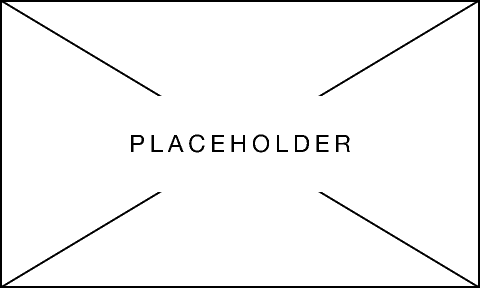
\includegraphics[width=\textwidth]{img/placeholder.png}
		\caption{Point contact model without friction.}
		\label{fig:pwof}
	\end{subfigure}
	\hfill
	\begin{subfigure}[b]{0.3\textwidth}
		\centering
		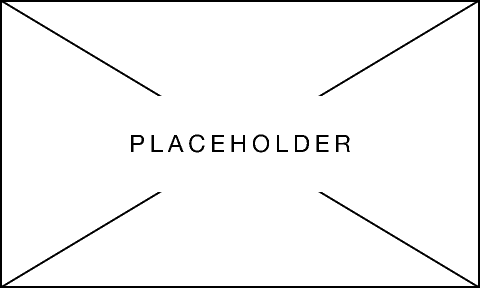
\includegraphics[width=\textwidth]{img/placeholder.png}
		\caption{Point contact model with friction.}
		\label{fig:hf}
	\end{subfigure}
	\hfill
	\begin{subfigure}[b]{0.3\textwidth}
		\centering
		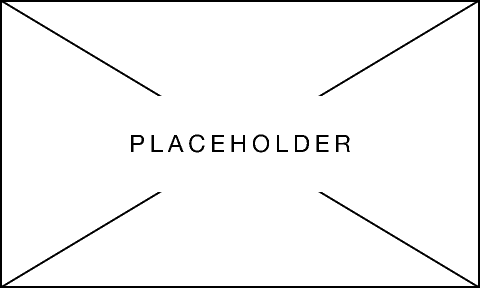
\includegraphics[width=\textwidth]{img/placeholder.png}
		\caption{Soft-finger model.}
		\label{fig:sf}
	\end{subfigure}
	   \caption{The three most commonly used contact models.}
	   \label{fig:contact-models}
\end{figure}

% no friction
The \gls{pwof} model, as shown in \figref{fig:pwof}, can only represent forces along with the normal of the object's surface at the point of contact and thus the model does not support surface deformations between the two contacting objects. This model is applied in cases where very little deformation is present along with the contact being slippery\cite[Chapter 38]{handbook-of-robotics}.\medskip

% Hard finger
The \gls{hf} model, as shown in \figref{fig:hf}, is representative when the friction between objects is great enough to be significant, while the contact deformation is small enough to ignore friction moments\cite[Chapter 38]{handbook-of-robotics}. To model the friction acting on the contact point a great number of methods exist, the most common being the Column friction with different modifications depending on the use case\fakecite. \medskip

% Soft finger
The \gls{sf} model, as shown in \figref{fig:sf}, is used to represent scenarios where both friction and surface deformations are great enough to be impactful in the systems behavior. Due to deformations of the finger an additional torsional moment about the contact normal will be present.
\cite[Chapter 38]{handbook-of-robotics}  \medskip


% draw the model as applied in our case

% subcategories of sf models
Based on the contact model categories described above, the most representative is \gls{sf} since these models can provide descriptions of the contact surface topology, and thus enable the solving of the \gls{iep} by deriving surface features for pose estimation. Within the category of \gls{sf} models a method fit for this project's use case is to be chosen to solve problem \ref{prob:1}. \gls{sf} models can furthermore be divided up into three different categories: \gls{aebm}, \gls{efm} and \gls{fem} \cite{a-modified-elastic-foundation-contact-model-for-application-in-3d-models-of-the-prosthetic-knee}. \medskip


% reformulate
% \gls{aebm} are theoretical formulations of elasticity calculating contact areas and stresses on both the surface and the sub-surface of the contacting bodies, but are restricted to simple geometries. The classical Hertz contact model (Hertz, 1882; Johnson, 1995)

% 

% 1) I want to model contacts
% 2) there exist 8 different modeling taxonolies
% 3) three are most common
% 	3.a) explain each of the three 
% 4) since soft supports the behavior we want we choose that one
% 5) what method categories exist within soft finger modelling



% In order to model the pressure distribution in the contact area different models have been devel-
% oped that fall into three main categories: analytical elasticity-based models, elastic foundation models
% (EFM) and finite element models (FEM) (Pérez-González et al., 2008). Analytical models are based on
% theoretical formulations of elasticity calculating contact areas and stresses on both the surface and the
% sub-surface of the contacting bodies, but are restricted to simple geometries. The classical Hertz con-
% tact model (Hertz, 1882; Johnson, 1995) and others derived from it are part of this category. However,
% robotic fingertips are made of nonlinear elastic materials. For that reason, the Hertzian contact model
% does not accurately represent this type of contact. EFMs were developed in order to allow a simple
% discrete contact calculation in more general surface geometries modelling the deformable part of the
% contact as a layer over a rigid base, and a series of discrete and independent springs in the contact
% normal direction. An application of this category of models is presented in Section 3.4 where it is used
% to create a simulation of a general tactile sensor and validated in robot grasping applications. FEMs
% have been increasingly used over recent years given that they supply information about the sub-surface
% stresses and strain in volumetric finite elements. However, they are excessively time consuming for fast
% simulation in dynamic grasping and manipulation models. Therefore, simplified numerical models are
% interesting alternatives.

% with friction



% soft finger


% When choosing a representative contact model, two overarching groups exist: linear and non linear models. While the linear models often are too simple to properly represent the real phenomena, their simplicity often make them a popular choice for practical reasons. \medskip

% Within the linear models group we find the most common model: The Hertzian contact model\cite*{on-the-contact-of-rigid-elastic-solids-and-on-hardness}. This model makes the assumptions that
% the objects consist of linear elastic materials when in contact and the contact deformations are small compared to the dimension of object.


% non-linear models

% When considering the non linear contact models, the simpler 

% The Hertzian contact model specifically assumed linear elastic objects in contact with small deformation. Later, the study of contact mechanics became a branch in mechanics. One of the important results in his seminal paper postulated that where N is the normal force, a is the radius of circular contact area, and C is a proportional constant. Equation (2), derived by Hertz [13], describes the growth of radius of circular contact area as proportional to the normal force raised to the power of 3 1 . It is important to note that Hertz had assumed that ( i ) the contact is linear elastic and ( ii ) the deformation is small.



% 

% \begin{center}
%     \renewcommand{\arraystretch}{1.2}
%     \begin{minipage}{.48\linewidth}
%         \vspace{0pt}
%         \centering
%         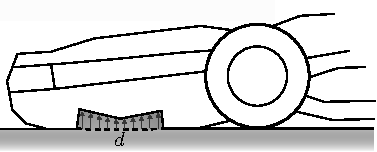
\includegraphics[width=.95\textwidth]{chapters/modeling/fig/measure-displacement.pdf}
%     \end{minipage}%
%     \vspace{15pt}
%     \begin{minipage}[t]{.48\linewidth}
%         \vspace{0pt}
%         \captionsetup{type=figure}
%         \captionof{figure}{The friction forces $\mathbf{f}_f$ and contact model keeps the object $\{O\}$ from slipping between the \gls{ee}'s fingers when the gravitational pull $\mathbf{f}_g$ is acting on it.}
%         \label{fig:measure-displacement}
%     \end{minipage}%
% \end{center}

% in order to perform tactile perception we need to model the contact between the end effector and the object of interest -> 
% 	This model needs to provide descriptions of parameters such as pressure and area for the contact to be 
% 	This model needs to contain the pressure and deformation caused by the contact in order to recreate the surface of contact





% What are contact models and what do they describe?
% For tactile perception it is needed to model the contact between the robotic manipulator finger and the object. The model will here 

% we need a model


%  what do we wish to model contact forces and how they can relate to deformation. Friction to determine how much force to apply in order to keep the object in the grasp.


%  


% flush out what exactly the model i want to use looks like


% When considering different methods for modeling contact interfaces, each can be categorized depending on which parameters the model describe the relation between. This results in the following groupings: contact-area-force models, stress-strain models, force-displacement models and 

% How are models grouped and what groupings exist?

% Contact models can be grouped based on the what parameters the relation is describing.







% Contact Area vs. Applied Force


% Hertzian contact model

% Soft Contact Model (More general Hertzian model)

% Viscoelastic Soft Contact Model.

% 	 Kelvin–Voigt/Maxwell model
% 	  Fung’s model

% Other contact models (research)



% Boussinesq–Cerruti’s

% Love’s solution 




% Love's formulation 




% What is tactile perception? Why is it relevant? \\
% How is a tactile sensor constructed \cite{recent-progress-in-technologies-for-tactile-sensors}
% what different types exist and which one is present in the model provided.


% \textit{"Representations of tactile data are commonly either inspired by machine vision feature descriptors"}

% often used in computer vision context, where each tactile image 

% Addressing the problem 





\section{Problem 2 - Pose Estimation} \label{sec:lit-rev-problem-2}

\section{Problem 3 - In-Hand Manipulation} \label{sec:lit-rev-problem-3}

\pagebreak
\chapter{Problem 1} \label{ch:problem1}


\section{Introduction} \label{sec:problem1-introduction}
Here we write the introduction for problem 1.


\section{Related Work} \label{sec:problem1-related-work}

Here we cite the related work by \texttt{\textbackslash cite\{source-label\}} like this \cite{recent-progress-in-technologies-for-tactile-sensors}

\pagebreak
\chapter{Problem 2} \label{ch:problem2}

\pagebreak
\chapter{Discussion} \label{ch:discussion}

\pagebreak
\chapter{Conclusion}\label{ch:conclusion}

this is the conclusion

% bibliography
\pagebreak
% \printbibliography[heading=bibintoc]
% \begin{multicols}{2}[\printbibheading]
% \printbibliography[heading=none]
% \end{multicols}
\printbibliography

\appendix
\chapter{Shadow Dexterous Hand - Technical Specifications}\label{app:shadow-dexterous-hand-technical-specifications}

\tabref{app:range-of-motion-shadow-hand} shows the \gls{rom} for the Shadow Dexterous Hand and \tabref{app:range-of-motion-human-hand} shown the \gls{rom} for a human hand. The shorthand abbreviations used in these tables can be seen listed in \tabref{app:joint-abbreviations}. The joints are numbered from fingertip to base and thus FF1 refers to the first joint after the fingertip on the first finger i.e. the index finger.
\begin{table}[!h]
\begin{center}
	\begin{tabular}{ |p{0.22\textwidth}|p{0.08\textwidth}|p{0.08\textwidth}|p{0.08\textwidth}|p{0.08\textwidth}|p{0.3\textwidth}| } 
	\hline
	\multicolumn{6}{|c|}{\textbf{\gls{rom} - Shadow Dexterous Hand}} \\ \hline
	\textbf{Joint(s)} & \textbf{Min deg} & \textbf{Max deg} & \textbf{Min rad} & \textbf{Max rad} & \textbf{Notes} \\ \hline
	FF1, MF1, RF1, LF1 &0&90&0&1.571  & \multirow{2}{4em}{Coupled}\\ \cline{1-5}
	FF2, MF2, RF2, LF2 & 0   & 90 & 0      & 1.571 & \\ \hline
	FF3, MF3, RF3, LF3 & -15 & 90 & -0.262 & 1.571 & \\ \hline
	FF4, MF4, RF4, LF4 & -20 & 20 & -0.349 & 0.349 & \\ \hline
	LF5&0&45&0&0.785 &  \\ \hline
	TH1&-15&90&-0.262&1.571 &  \\ \hline
	TH2&-40&40&-0.698&0.698 &  \\ \hline
	TH3&-12&12&-0.209&0.209 &  \\ \hline
	TH4&0&70&0&1.222& \\ \hline
	TH5&-60&60&-1.047&1.047& \\ \hline
	WR1&-40&28&-0.698&0.489& \\ \hline
	WR2&-28&10&-0.489&0.174& \\ \hline
	\end{tabular}
	\caption{The ranges of motion for each joint in the Shadow Dexterous Hand~\cite{range-of-motion-shadow-hand}.}
	\label{app:range-of-motion-shadow-hand}
\end{center}
\end{table}

\begin{table}[!h]
	\begin{center}
		\begin{tabular}{ |p{0.22\textwidth}|p{0.08\textwidth}|p{0.08\textwidth}|p{0.08\textwidth}|p{0.08\textwidth}|p{0.3\textwidth}| } 
		\hline
		\multicolumn{6}{|c|}{\textbf{\gls{rom} - Human Hand}} \\ \hline
		\textbf{Joint(s)} & \textbf{Min deg} & \textbf{Max deg} & \textbf{Min rad} & \textbf{Max rad} & \textbf{Latin Name} \\ \hline
		TH1 & -15 & 80 & & & Interphalangeal (IP) \\ \hline
		TH2 + TH3 & -10 & 55 & & & Metacarpophalangeal (MCP)\\ \hline
		TH4 +TH5  & -10 & 55 & & & Carpometacarpal (CMC)\\ \hline
		FF1, MF1, RF1, LF1 & 0 & 80 & & & Distal interphalangeal (DIP) \\ \hline
		FF2, MF2, RF2, LF2 & 0 & 100 & & & Proximal interphalangeal (PIP) \\ \hline
		FF3, MF3, RF3, LF3 & -45 & 90 & & & Metacarpophalangeal (MCP) \\ \hline
		WR1 &-80&80& & & Radiocarpal \\ \hline
		WR2 &-28&20& & & Radiocarpal \\ \hline
		\end{tabular}
		\caption{The theoretical \gls{rom} for each finger joint in human hand~\cite{continuous-and-simultaneous-estimation-of-finger-kinematics-using-inputs-from-an-emg-to-muscle-activation-model} and found \gls{rom} for the wrist joints~\cite{functional-wrist-motion:-a-biomechanical-study}.}
		\label{app:range-of-motion-human-hand}
	\end{center}
\end{table}

\begin{table}[!h]
	\begin{center}
		\begin{tabular}{ |l|l| } 
		\hline
		\multicolumn{2}{|c|}{\textbf{Joint Name Abbreviation}} \\ \hline
		\textbf{Abbreviation} & \textbf{Full Name} \\ \hline
		FF & First Finger \\ \hline 
		MF & Middle Finger \\ \hline 
		RF & Ring Finger \\ \hline 
		LF & Little Finger \\ \hline 
		WR & Wrist \\ \hline 
		\end{tabular}
		\caption{The abbreviations used to reference ~\cite{joint-abbreviations-shadow-hand}.}
		\label{app:joint-abbreviations}
	\end{center}
	\end{table}

To compare the kinematic structure of the Shadow Dexterous Hand and a human hand, see~\figref{app:human-and-robot-hand-kinematics}.

\begin{figure}[!h]
	\centering
	\begin{subfigure}[b]{0.3\textwidth}
		\centering
		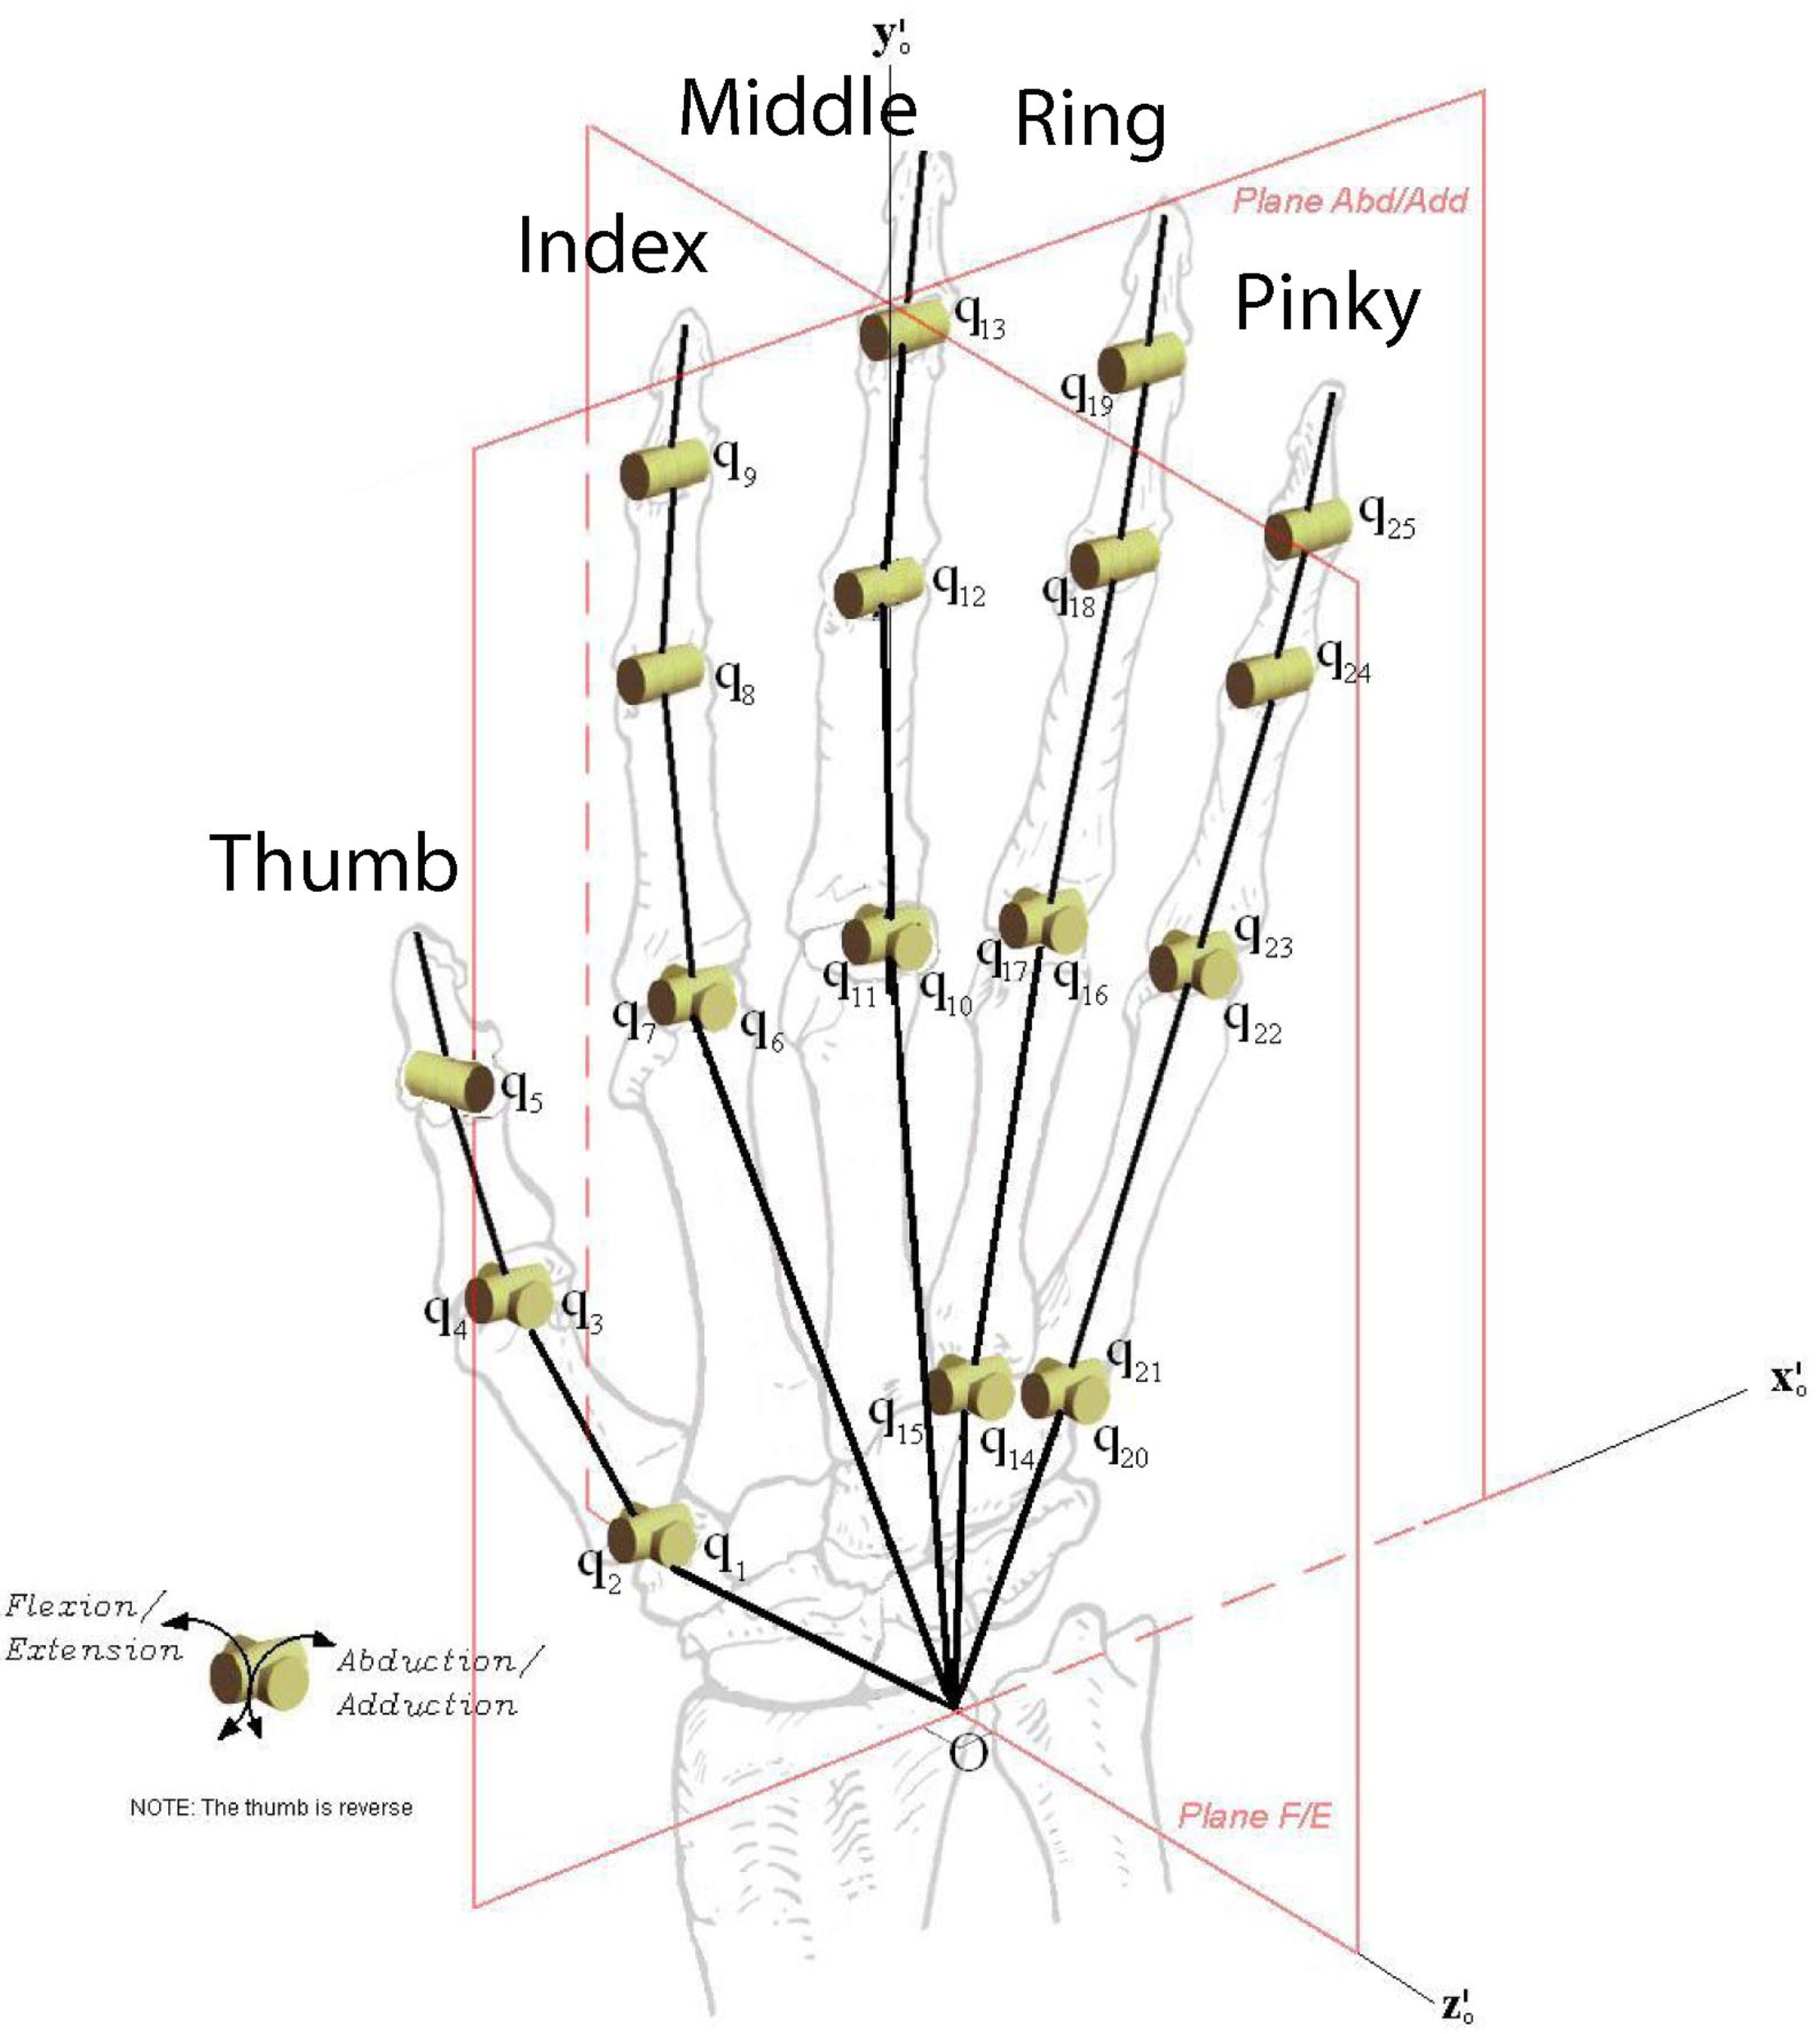
\includegraphics[width=\textwidth]{chapters/appendix/fig/human-hand-kinematics.pdf}
		\caption{The kinematic tree of a human hand according to~\cite{grasp-synthesis-algorithms-for-multifingered-robot-hands}.}
		\label{app:human-hand-kinematics}
	\end{subfigure}
	\hfill
	\begin{subfigure}[b]{0.69\textwidth}
		\centering
		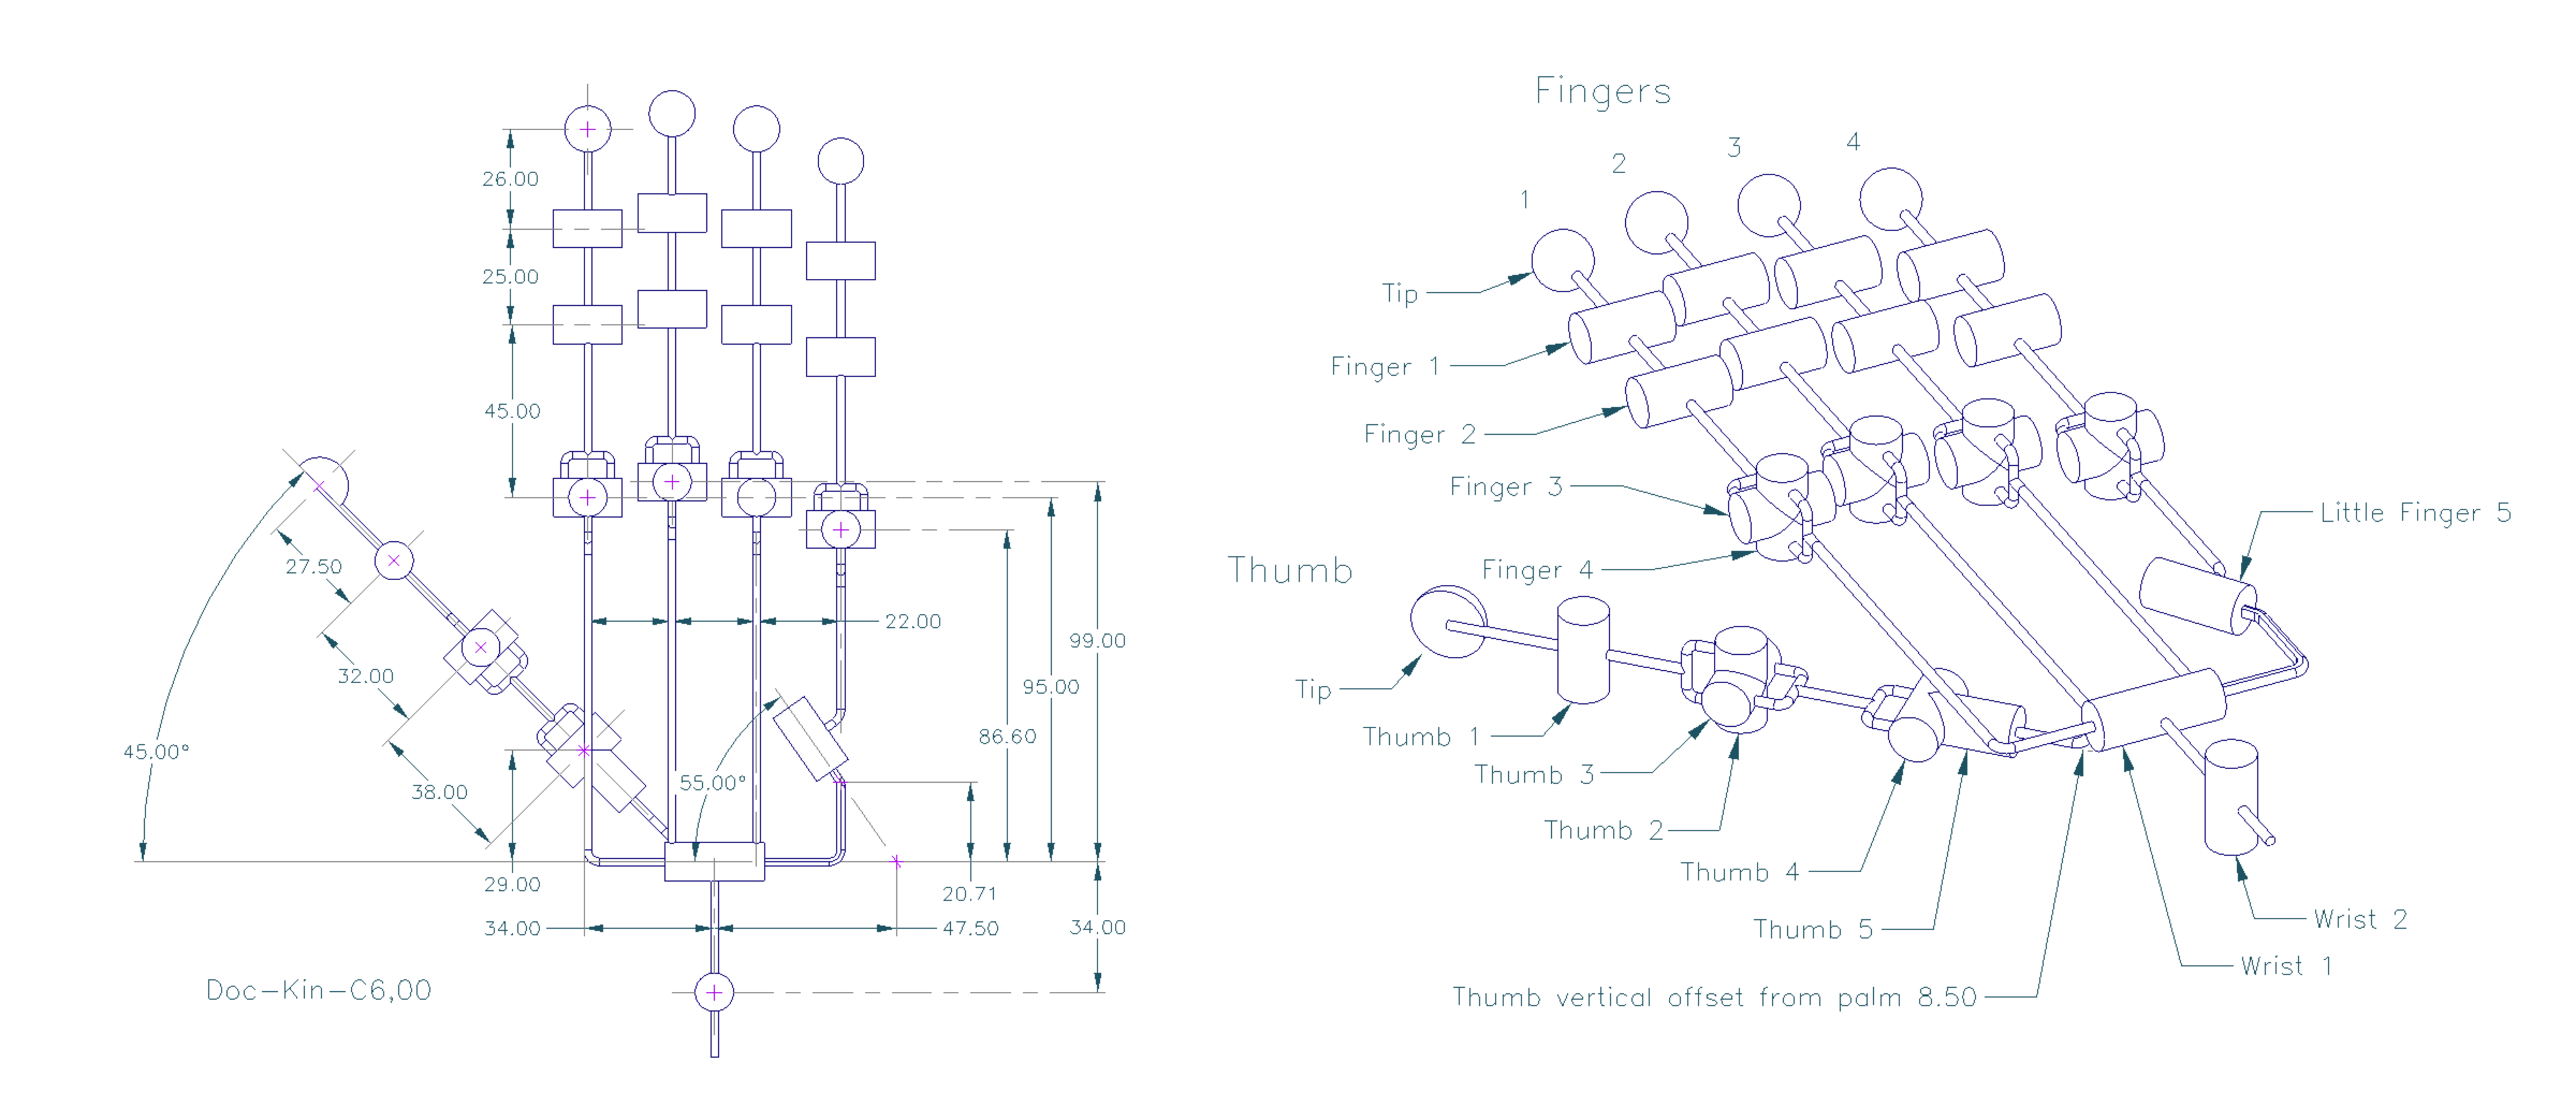
\includegraphics[width=\textwidth]{chapters/appendix/fig/robot-hand-kinematics.pdf}
		\caption{The kinematic tree of the Shadow Dexterous Hand according to~\cite{robot-hand-kinematics}. \newline}
		\label{app:robot-hand-kinematics}
	\end{subfigure}
	\caption{The kinematic trees of a human hand and the Shadow Dexterous hand.}
	\label{app:human-and-robot-hand-kinematics}
\end{figure}

\chapter{Tactile Perception - Simulated Electrode Activations}\label{app:tactile-perception-simulated-electrode-activations}

Below three 

\begin{figure}[!h]
	\begin{center}
		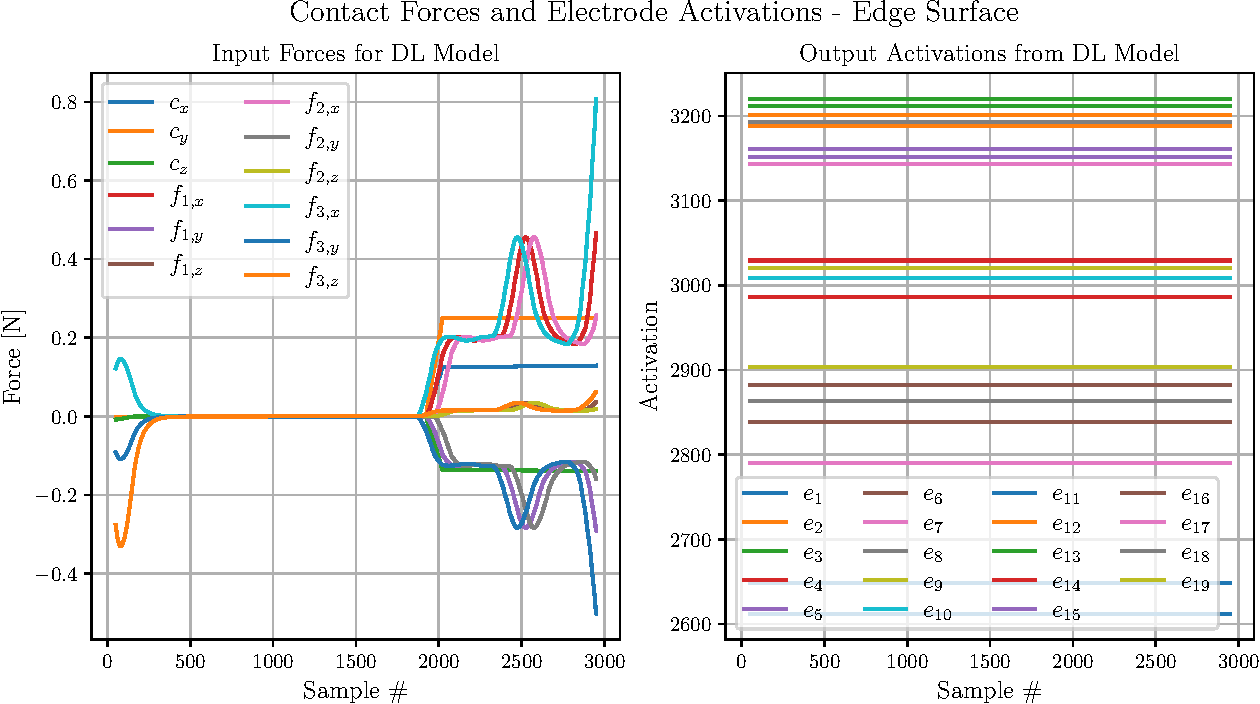
\includegraphics[width=\textwidth]{chapters/1-tactile-perception/fig/matplotlib/edge-contact-graph.pdf}
	\end{center}
	\caption{he simulated tactile electrode activations when the simulated Shadow Dexterous hand's index finger is in contact with an edge.}
	\label{app:edge-contact-graph}
\end{figure}

\begin{figure}[!h]
	\begin{center}
		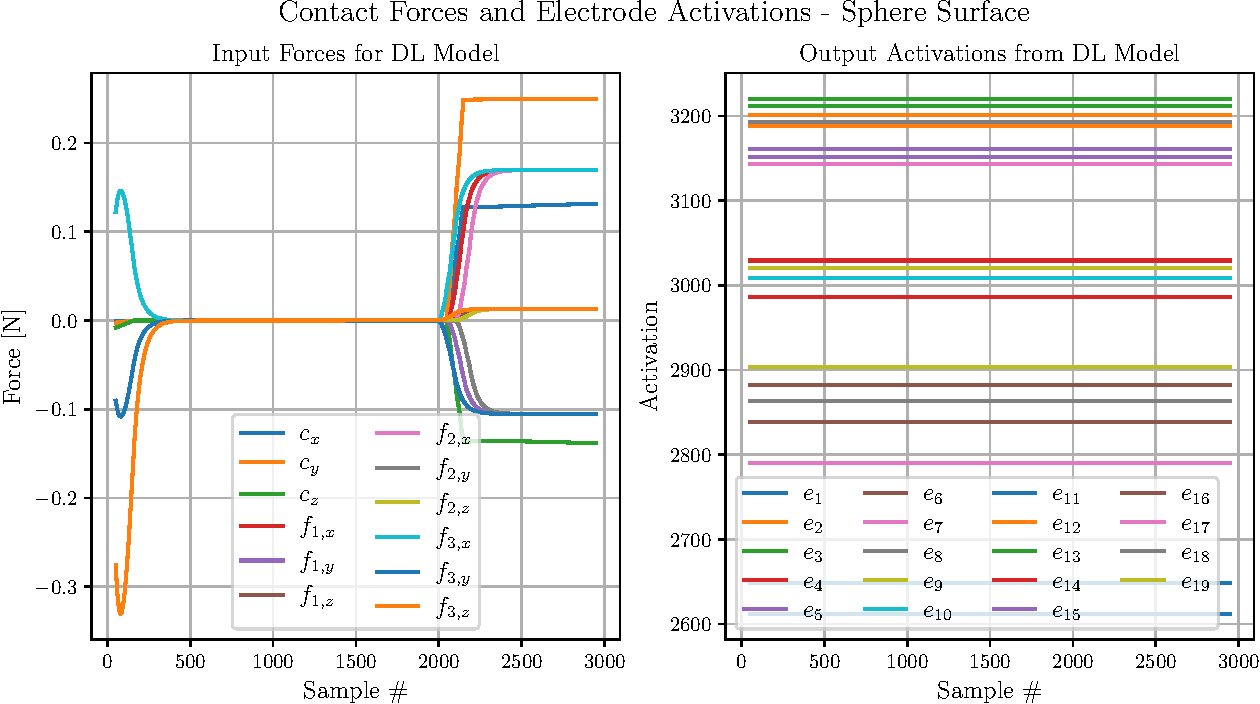
\includegraphics[width=\textwidth]{chapters/1-tactile-perception/fig/matplotlib/sphere-contact-graph.pdf}
	\end{center}
	\caption{The simulated tactile electrode activations when the simulated Shadow Dexterous hand's index finger is in contact with a smooth surface.}
	\label{app:smooth-contact-graph}
\end{figure}

\begin{figure}[!h]
	\begin{center}
		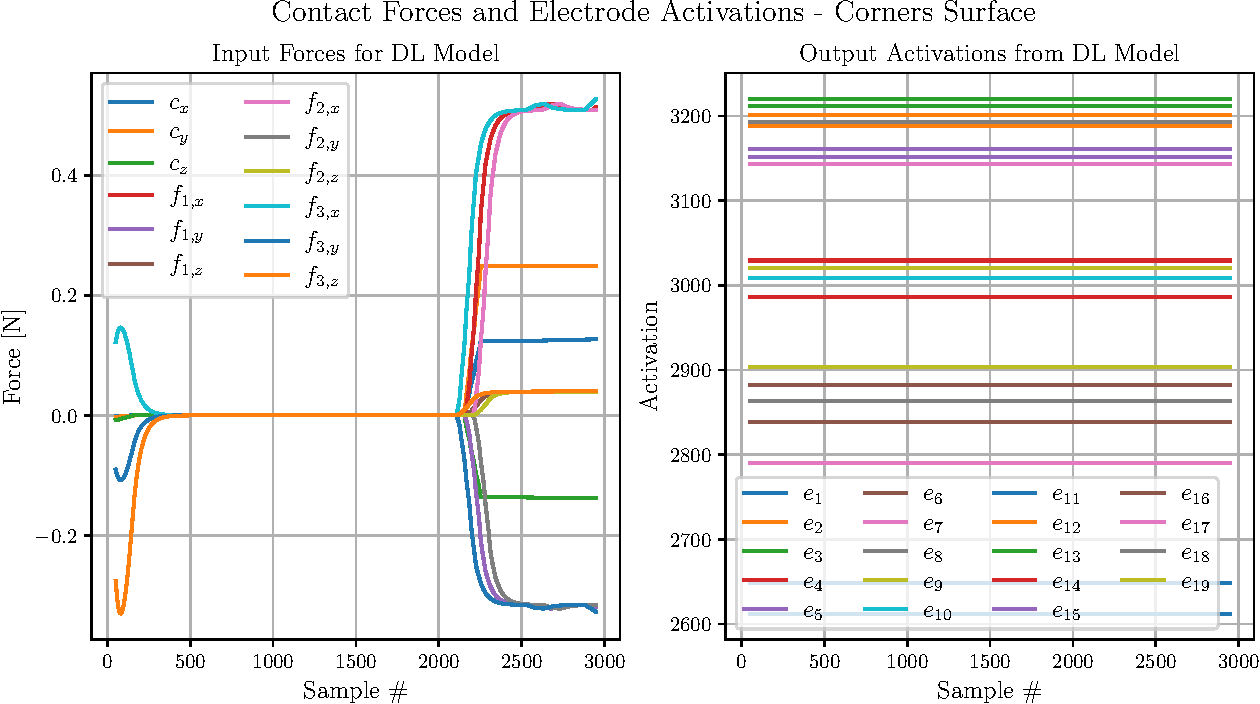
\includegraphics[width=\textwidth]{chapters/1-tactile-perception/fig/matplotlib/corners-contact-graph.pdf}
	\end{center}
	\caption{The simulated tactile electrode activations when the simulated Shadow Dexterous hand's index finger is in contact with a corner.}
	\label{app:corner-contact-graph}
\end{figure}

\end{document}